\documentclass[11pt,oneside,a4paper]{article}
\usepackage{graphicx}
\usepackage{booktabs}
\usepackage{caption}
\usepackage{subcaption}
\usepackage{amsmath}
\usepackage{amsfonts}
\usepackage{amssymb}
\usepackage{lscape}
\usepackage{psfrag}
\usepackage[usenames]{color}
\usepackage{bbm}
\usepackage[update]{epstopdf}
\usepackage[bookmarks,pdfstartview=FitH,a4paper,pdfborder={0 0 0}]{hyperref}
\usepackage{verbatim}
\usepackage{listings}
\usepackage{textcomp}
\usepackage{fancyhdr}
\usepackage{multirow}
\usepackage{tikz}
\usepackage{lipsum}
\usepackage{xcolor}
\usepackage{wrapfig}
\usepackage[margin=1in]{geometry}
\usepackage{pdfpages}
\newcommand{\hint}[1]{{\color{blue} \em #1}}

\makeatletter
\def\cleardoublepage{\clearpage\if@twoside \ifodd\c@page\else%
\hbox{}%
\thispagestyle{empty}%
\clearpage%
\if@twocolumn\hbox{}\clearpage\fi\fi\fi}
\makeatother

\sloppy
% \widowpenalty=10000
% \clubpenalty=10000

\title{
    \vspace*{0.0mm}
    \LARGE\bf\sf Network Security (Fall 2019)
    \vspace*{10.0mm} \\
    %
    \Huge\bf\sf Summary
    %
    \vspace*{30.0mm} \\
    \normalsize
    %
    \sf Author:\\[5pt]
    \sf Yannick Merkli\\ [5pt]
    \sf \pageref{lastpage} Pages
}
\date{}

\begin{document}

\maketitle
\thispagestyle{empty}
\raggedbottom
\clearpage

\pagenumbering{roman}

\clearpage
\setcounter{tocdepth}{2}
\tableofcontents
\clearpage
\pagenumbering{arabic}

\begin{center}
	\noindent \textbf{\LARGE Disclaimer: Legal use of the material}
	
	\noindent Some knowledge, technologies, code is usable for attacks, it is illegal to use them for criminal activities. It is also illegal to make available such technologies and code without proper measures.\\
	This summary is based on \cite{netsec}.
\end{center}


\newpage

\section{SSL, TLS, PKI}

\subsection{SSL/TLS Overview}

Goal: Secure Internet communication.\\
We need \textit{secrecy} to precent eavesdroppers from learning sensitive information and we need entity and message authentication to prevent message alteration/ injection.

\subsection{PKI overview}

In symmetric cryptography, main challenge is key distribution as keys need to be distributed via confidential and authentic channels. In public-key systems, main challenge is key authentication (i.e., which key belongs to whom) as keys need to be distributed via authentic channels.\\
\textit{Public-key infrastructures (PKIs) provide a way to validate public keys}.\\

\noindent Terminology: 

\vspace{-\topsep}
\begin{itemize}
	\setlength{\itemsep}{0pt}
	\setlength{\parskip}{0pt}
	\item PKI: Public-key infrastructures
	\item CA: Certification authority
	\item A public-key certificate (or simply certificate) is signed and binds a name to a public key \item Trust anchor, trust root: self-signed certificates of public keys that are allowed to sign other certificates.
	\item X.509: standard format of digital certificate, defines a structure for public key certificates: Two sections: data and signature section.
\end{itemize}
\vspace{-\topsep}

\noindent Trust establishment: You cannot establish trust out of thin air - we need a root of trust to establish trust in other entities. Cryptographic operations enable transfer of trust from one entity to another.

\subsection{X.509}

X.509 defines a structure for public key certificates

\vspace{-\topsep}
\begin{itemize}
	\setlength{\itemsep}{0pt}
	\setlength{\parskip}{0pt}
	\item Two sections: data and signature sec1on
	\item A CA assigns a unique name to each user and issues a signed certificate
	\item Often name is the domain or Email address
	\item Each CA issues a certificate for those beneath it
\end{itemize}
\vspace{-\topsep}

\noindent Multi-Domain Certificates are possible and used e.g. by CDNs. Content Delivery Networks (CDN) are hosting web sites for domains and thus need a certificate to service content. CDNs are obtaining a single certificate for multiple domains.

\subsection{Compelled Certificates}

Compelled certificate: public/private key pair for law enforcement (MitM attacks on TLS) with CA certificate enabling private key to sign additional certificates. Compelled certificates carry inherent risks: Since the certificates are non-repudiable, anyone who gets hold of the second valid certificate the CA's or the government's involvement in a compelled certificate creation attack. This results in a loss of trust in the CA or the government. If the CA creates an intermediary CA certificate for the government, then that certificate would have to be registered in a CT log, but in that case, the attack
does not become directly attributable to VeriSign, as the forged certificate is signed by the intermediary certificate.

\newpage

\subsection{Approaches to improve TLS}

\subsubsection{The “Let’s Encrypt” CA}

Goal: provide free certificates with automatic domain validation, issuance, and renewal. It uses relatively short-lived certificates (90 days). It is based on ACME (Automated Certificate Management Environment).

\subsubsection{Levels of trust}

Have different levels of trust in certificates:

\vspace{-\topsep}
\begin{itemize}
	\setlength{\itemsep}{0pt}
	\setlength{\parskip}{0pt}
	\item No SSL/TLS
	\item Domain validation (DV): the domain is validated but the owner could be malicious (e.g. bad.com with certificate for bad.com)
	\item Organization validation (OV) / "High assurance": A certificate provider will issue an OV class certificate to a purchaser if the purchaser can meet two criteria: the right to administratively manage the domain name in question, and perhaps, the organization's actual existence as a legal entity. (e.g. wikipedia.org)
	\item Extended validation (EV): can be issued only by a subset of certificate authorities (CAs) and require verification of the requesting entity's legal identity before certificate issuance (e.g. credit-suisse.com). They are further displayed differently in most browsers. 
\end{itemize}
\vspace{-\topsep}

\subsubsection{HTTP Strict Transport Security (HSTS)}

Goal: allows servers to declare that their clients should only use HTTPS (for a specified period). This prevents some “downgrade”, “SSL stripping”, and “session hijacking” attacks. Browsers should automatically redirect to HTTPs or display a warning message. HSTS is implemented with an HTTPS header. Example: \\
\indent \texttt{Strict-Transport-Security: max-age=31536000}\\
\noindent HSTS doesn't help at all if valid bogus certificates are used.

\subsubsection{HTTP Public-Key Pinning (HPKP)}

A server implementing HPKP will provide the client with a list of hashes of valid
certificates for the domain. This list is delivered in an HTTP header that also contains a
max-age value. The client will then “pin” those hashes — subsequent connection within the
max-age period will only succeed if the certificate offered by the server matches the pinned
hashes for that domain. A MitM with a different certificate would therefore fail. Example:\\
\indent \texttt{Public-Key-Pins: max-age=2592000; pin-sha256="..."; pin-sha256="...";\\
	\indent report-uri="...";\\
}
MiTM attacks can still succeed even with HPKP: HPKP is TOFU (Trust On First Use). If the first policy received comes from an
attacker, the browser will be happy to communicate with the bogus website and will block
the legitimate server. Also if a weak hash function is used, the attacker could generate a
certificate with a colliding hash — but in that case HPKP would be the last of our problems.\\

\noindent Further problem with HPKP: certificates can change often (e.g with Let's encrypt). If a certificate changes but users still hold the old policy (since the max-age hasn't expired yet), clients won't accept the new certificate although it is legitimate.

\newpage

\subsubsection{Certificate revocation}

Certificate revocation is a mechanism to invalidate certificates (e.g. after a private key is disclosed or after a trusted employee leaves a company). CA periodically publishes certificate revocation List (CRL).\\
Problem: CAP theorem (Consistency, Availability, tolerance to Par11on):
impossible to achieve all 3, need to sacrifice one!

\subsubsection{Online Certificate Status Protocol (OCSP)}

Online Certificate Status Protocol (OCSP) to verify certificate status, ensure certificate is valid and has not been revoked. Browsers will send certs to OCSP server for verification.\\
Problem: 
\vspace{-\topsep}
\begin{itemize}
	\setlength{\itemsep}{0pt}
	\setlength{\parskip}{0pt}
	\item “Optimistic” treatment of OCSP failure information: If OCSP server does not respond, a certificate would be considered invalid, although the certificate most likely isn't. This leads to false positives, which is annoying for browser users, that's why most browsers don't treat a non-responding OCSP server as invalid certificate.
	\item OCSP servers can be slow, which is another reason for browsers to deactivate it by default, since users otherwise may switch browsers.
	\item OCSP can leak browsing information outside of private browsing mode as Microsoft’s CryptoAPI and Apple’s Security Framework API cache OCSP responses in OS.
\end{itemize}
\vspace{-\topsep} 

\noindent Possible solution: OCSP stapling allows the presenter of a certificate to bear the resource cost involved in providing OCSP responses by appending ("stapling") a time-stamped OCSP response signed by the CA to the initial TLS handshake, eliminating the need for clients to contact the CA, with the aim of improving both security and performance.

\subsubsection{DNS-Based Authentica1on of Named Entities (DANE)}

Goal: authenticate TLS servers without a certificate authority (CA). DANE uses DNSSEC to bind certificates to names. Problem: this is heavily reliant on DNSSEC.

\subsubsection{Attack-resilient PKI (ARPKI)}

Goal: reduce trust in any single component (e.g. CA, log server, etc.). Reduce attack surface, no single point of failure.\\
ARPKI has a set of entities that audit each other's operation and disseminate misbehavior if detected:

\vspace{-\topsep}
\begin{itemize}
	\setlength{\itemsep}{0pt}
	\setlength{\parskip}{0pt}
	\item Client (browser) establishes TLS connections with	Domain
	\item Integrity Log Server (ILS) logs domains’ certificates, makes logs publicly available and maintains Integrity Tree
	\item Certification Authority (CA) certifies domains’ public keys, download ILS data and check consistency and check behavior of other CAs.
\end{itemize}
\vspace{-\topsep}

\noindent ARPKI communication flows:

\vspace{-\topsep}
\begin{itemize}
	\setlength{\itemsep}{0pt}
	\setlength{\parskip}{0pt}
	\item Domains obtain certificate with multiple signatures from different CAs
	\item CAs also act as validators to survey operation by ILSes. They download accepted requests and validate log
	\item $n$ parties are needed for valid certificate (ILS and $n-1$ parties are different CAs)
\end{itemize}
\vspace{-\topsep}

\begin{figure}[t!]
	\centering
	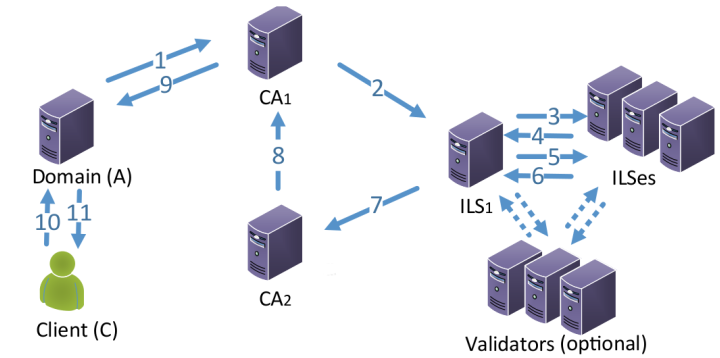
\includegraphics[width=0.5\linewidth]{figures/arpki}
	\caption{ARPKI}
	\label{fig:arpki}
\end{figure}

\newpage

\subsubsection{Certificate transparency (CT)}

Certificate	Transparency will make all public end-entity TLS certificates public knowledge,	and	will hold CAs publicly accountable for all certificates they issue. And it will do so without introducing another trusted third party.\\
\noindent CT uses a CT log that is an append-only list of certificates. The log server verifies the certificate chain (CA attribution for certificate miss-issuance and spam control). Periodically, all new certificates are appended to the append-only log and that list is then signed. All updates of the signed list of certificates ("the log") are published to the world. The CT log is implemented as a merkle hash tree. We have three participants in the protocol:

\begin{figure}
	\centering
	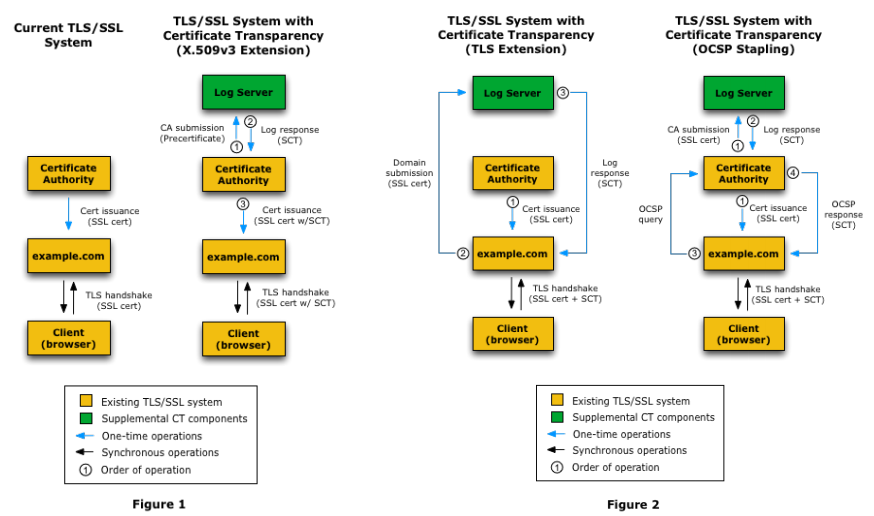
\includegraphics[width=0.9\linewidth]{figures/tls_with_ct}
	\caption{TLS with certificate transparency}
	\label{fig:tlswithct}
\end{figure}


\vspace{-\topsep}
\begin{itemize}
	\setlength{\itemsep}{0pt}
	\setlength{\parskip}{0pt}
	\item Log Server. Contains a list of certificates that is publicly available. Must
	add the certificates submitted by the CAs.
	\item Clients (auditors). Can verify the existence of certificates by checking the log server,
	and exchange information with the monitors about the log server status, in order to
	ensure the log server is not compromised.
	\item CAs (monitors). Request the addition of every newly issued cert, check that the log
	server actually adds the certificates, monitor what the other CAs are doing.
	\item Certificate owners: Query monitors to verify that nobody has logged illegitimate certs for their domain.
\end{itemize}
\vspace{-\topsep}

\newpage

\noindent Upon receiving a new certificate chain from domain or CA: the log verifies the certificate, issues a signed certificate timestamp (SCT) and promises to add the new certificate to the MHT (SCT is necessary since certs are only periodically added to log).\\
How does CT handle revocation? The certificates stay on the log forever: Merkle trees allow for easy insertion but not for immediate deletion. The current system implements revocation transparency, which is very similar to CT, but for revocation requests.\\

\noindent Disadvantages of CT:

\vspace{-\topsep}
\begin{itemize}
	\setlength{\itemsep}{0pt}
	\setlength{\parskip}{0pt}
	\item MitM attack still proceeds (but can be detected externally)
	\item Browser still needs to contact Log eventually to verify that certificate is listed in log
	\item Malicious Log server can add bogus certificate
\end{itemize}
\vspace{-\topsep}

\begin{figure}[hb]
	\centering
	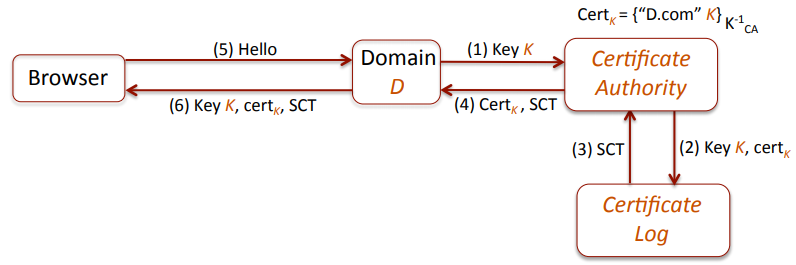
\includegraphics[width=0.6\linewidth]{figures/ct_summary}
	\caption{CT summary}
	\label{fig:ctsummary}
\end{figure}

\begin{figure}[hb]
	\centering
	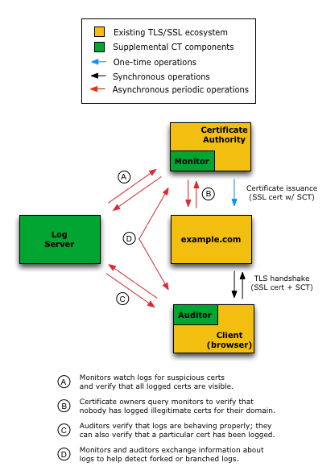
\includegraphics[width=0.5\linewidth]{figures/ct_participants}
	\caption{CT participants}
	\label{fig:ctparticipants}
\end{figure}











\label{lastpage} % this must stay here
\clearpage
\addcontentsline{toc}{section}{References}
\bibliographystyle{acm}
\bibliography{refs}

\clearpage
\appendix
\pagenumbering{Roman}

\end{document}
